\section{Dataset} \label{dataset}
This paper builds on data captured by TTNet \cite{voeikov2020ttnet} and released by OSAI \cite{OSAI}. The data includes match and player statistics from Tischtennis-Bundesliga, the top professional German table tennis league, as well as men and women's singles matches from the Tokyo 2020 Olympics. Many potential features such as player age, rank, match duration as well as in-match statistics such as percentage of points won on serve and receive, stroke types and error types are available. Interactive maps that demonstrated the ball position of each shot on the table, as well as the stroke type were also accessible (e.g. see Figure \ref{fig1}).

%\denes{Can we say that one of the challenges is to find out which features might be salient for a result predictor?}

\begin{figure}[ht]
\centering

%\vspace{-2em}
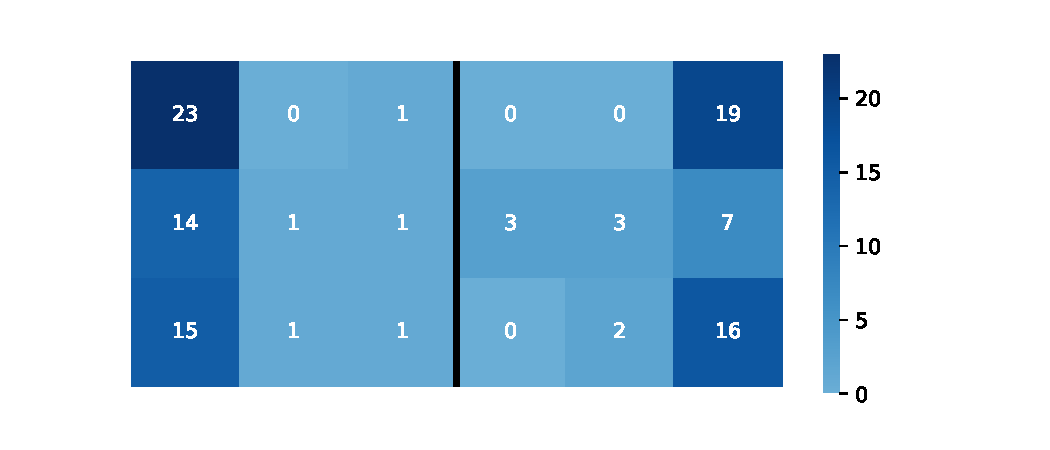
\includegraphics[width=8cm]{plots/tableheatmaprot.pdf}
\caption{Distribution of ball placement of a winning shot for both players by region if each side of the table were to be split into nine equal parts. Each value indicates the number of balls landing in it's respective region \cite{OSAI}.}

\label{fig1}
\end{figure}

\begin{figure}[ht]
\centering

%\vspace{-2em}
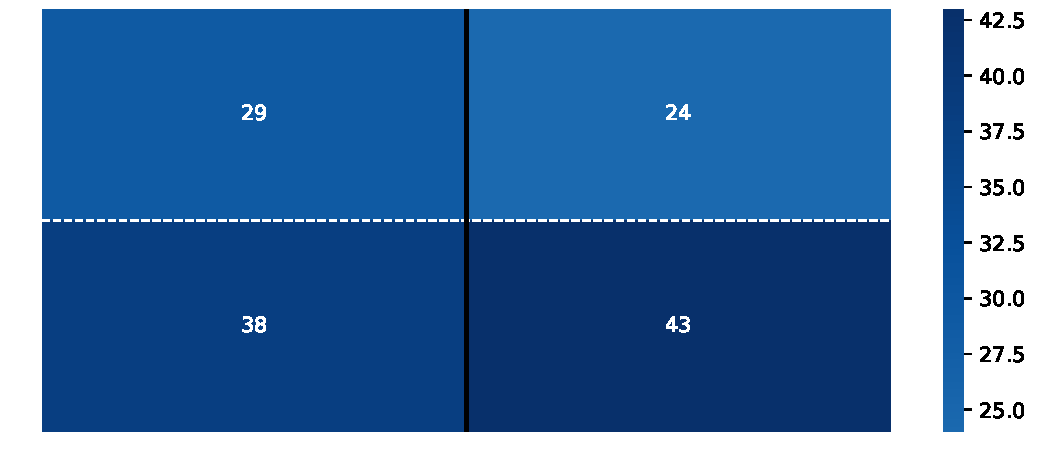
\includegraphics[width=8cm]{plots/forehandvsbackhand.pdf}
\caption{Distribution of rallies won on a forehand compared to a backhand}

%\vspace{-1.5em}
\label{fvbh}
\end{figure}

\begin{figure}[ht]
\centering

%\vspace{-2em}
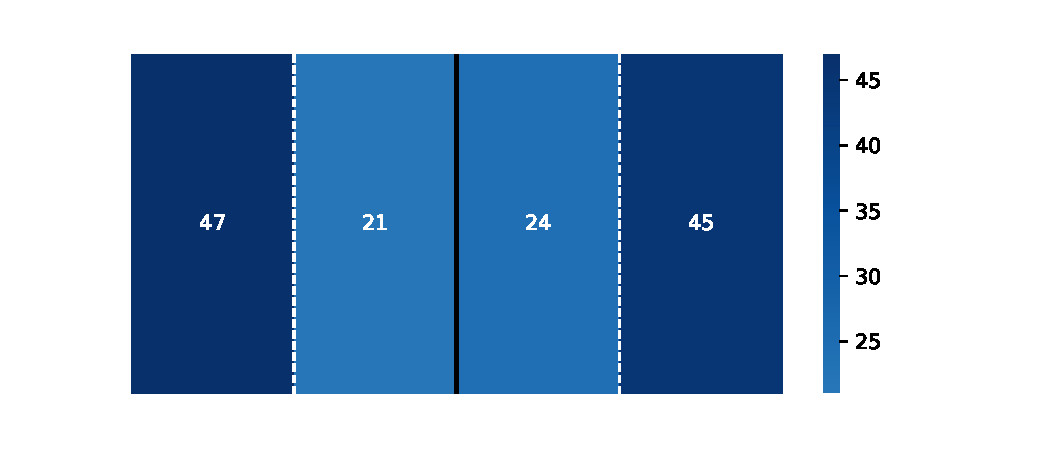
\includegraphics[width=8cm]{plots/shortvslongrally.pdf}
\caption{Distribution of points won on a short rally compared to a long rally}

%\vspace{-1.5em}
\label{svlr}
\end{figure}

\begin{figure}[ht]
\centering

%\vspace{-2em}
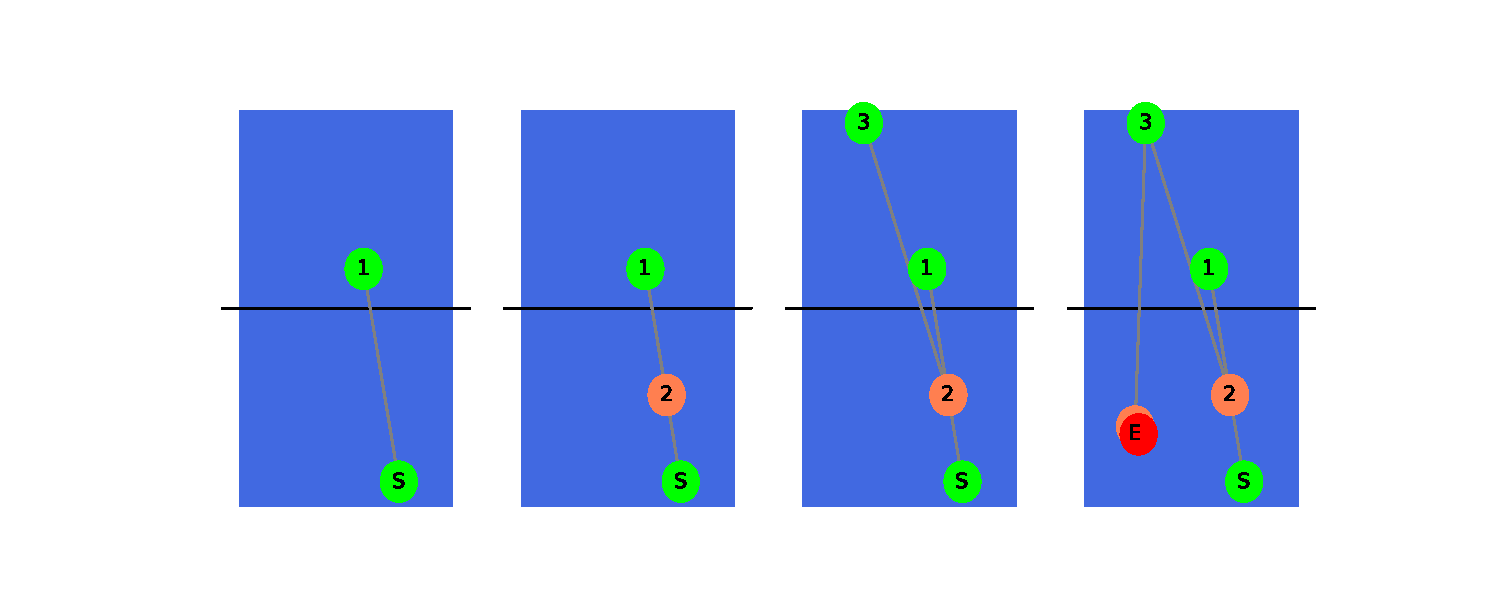
\includegraphics[width=8.5cm]{plots/tablesequence.pdf}
\caption{Rally Sequence}

%\vspace{-1.5em}
\label{sequence}
\end{figure}

 Samples with missing data entries were removed from the dataset. One of the main challenges in constructing a successful result predictor is the selection of salient features. To address this, we carefully hand picked features that we thought would be the most influential in a match based on existing domain knowledge on the problem.